\chapter{Modelado del problema}
\label{chap5}
\ifpdf
  \graphicspath{{Chapter5/Chapter5Figs/PNG/}{Chapter5/Chapter5Figs/PDF/}{Chapter5/Chapter5Figs/}}
\else
  \graphicspath{{Chapter5/Chapter5Figs/EPS/}{Chapter5/Chapter5Figs/}}
\fi

\markboth{\hfill \thechapter. Modelado del problema}{\hfill \thechapter. Modelado del problema}

\section{Planteamiento del problema}
% \label{cap:planteamiento}

La fase de recolección de residuos sólidos cumple un rol importante en los aspectos socio-económicos y ambientales de una ciudad. Según la literatura, gran parte del presupuesto de un municipio va destinada a dicha fase. En consecuencia, se genera la necesidad de una búsqueda permanente por disminuir costos en sus procesos sin afectar la calidad del servicio. 

Hoy en día, la selección de la ruta de recolección se basa en la propia intuición y experiencia de los conductores. En algunas ocasiones esto conlleva a dejar sin servicio algunos puntos de la ciudad por desconocimiento de un nuevo conductor asignado a la zona, que a su vez genera que la comuna asuncena realice quejas acerca de la falta de servicio de recolección en tiempo y forma. También es posible el paso en repetidas veces de forma innecesaria por la misma calle dando lugar a mayores gastos de combustible, como se indica en los círculos rojos de la Figura \ref{fig:trayectoRecoleccion}.

\begin{figure}[tb]
    \centering
    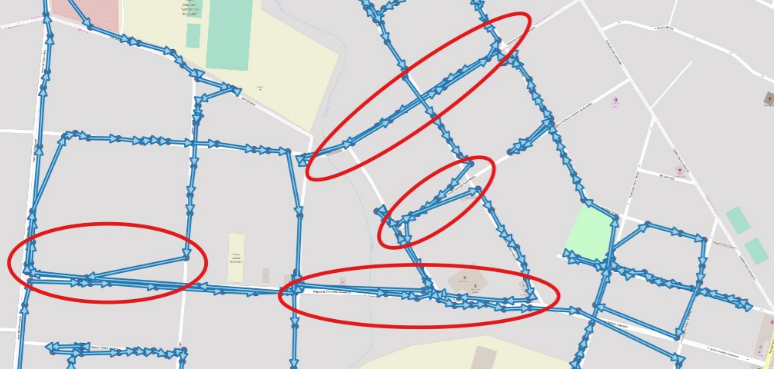
\includegraphics[width=14.5cm]{20170329_recorrido_repetido.png}
    \caption{Trayecto del vehículo 62 en fecha 11 de Julio del 2016 en el turno mañana. [Fuente: Datos de rastreo vía GPS desplegados en la aplicación QGis]}
    \label{fig:trayectoRecoleccion}
\end{figure}

Otra situación muy común es el frecuente cambio de circulación en las calles buscando disminuir la congestión del tráfico actual, por ejemplo: cambio de sentido, prohibición de giro a la izquierda, prohibición de giro en U, contramano. También se presentan situaciones donde las calles quedan clausuradas para su uso por motivo de reparación de la capa asfáltica, trabajos de instalación o reparación de cañería.

Por ello se evidencia la necesidad de una herramienta de soporte de decisión que aborde el problema del enrutamiento de los vehículos recolectores teniendo en cuenta el procedimiento actual llevado a cabo para la recolección de residuos domiciliarios de la DSU.

% Para  ello  se  implementa  una  solución  GIS  que  optimice  el  camino  del  vehículo recolector teniendo en cuenta el procedimiento actual llevado a cabo para la recolección de residuos domiciliarios, gestionando de forma sencilla y rápida el estado actual de las calles y sus reglas de circulación.

% En la Figura \ref{fig:trayectoRecoleccion}, se muestra una pequeña parte del rastreo de una zona, en los círculos de color rojo se pueden observar como el mismo vehículo recorre la misma calle más de una vez. Esta situación se pudo contemplar en los recorridos de varias zonas. Para la recolección de datos se solicitó a la DSU el permiso de instalar un dispositivo GPS a un vehículo recolector de basura, como parte de este proyecto, a través del cual obtuvimos por un periodo de 3 meses los datos de posicionamiento relacionados al vehículo 62 de propiedad de la Municipalidad de Asunción. Esta idea ya generó el interés de la Municipalidad de Asunción, que posteriormente ha realizado una licitación para dotar a todos los vehículos recolectores de residuos un dispositivo similar GPS, brindándonos acceso a los datos del rastreo de todos vehículos recolectores.

\section{Metodología de trabajo}

En la Figura \ref{fig:metodologia} se muestra la metodología seguida en este trabajo: la recolección de datos, selección de un modelo matemático adecuado para resolver el problema de ruteo, la implementación de la herramienta \textit{TapeYty}, el despliegue de la ruta óptima y por último el análisis de los resultados.

\begin{figure}[H]
\centerline{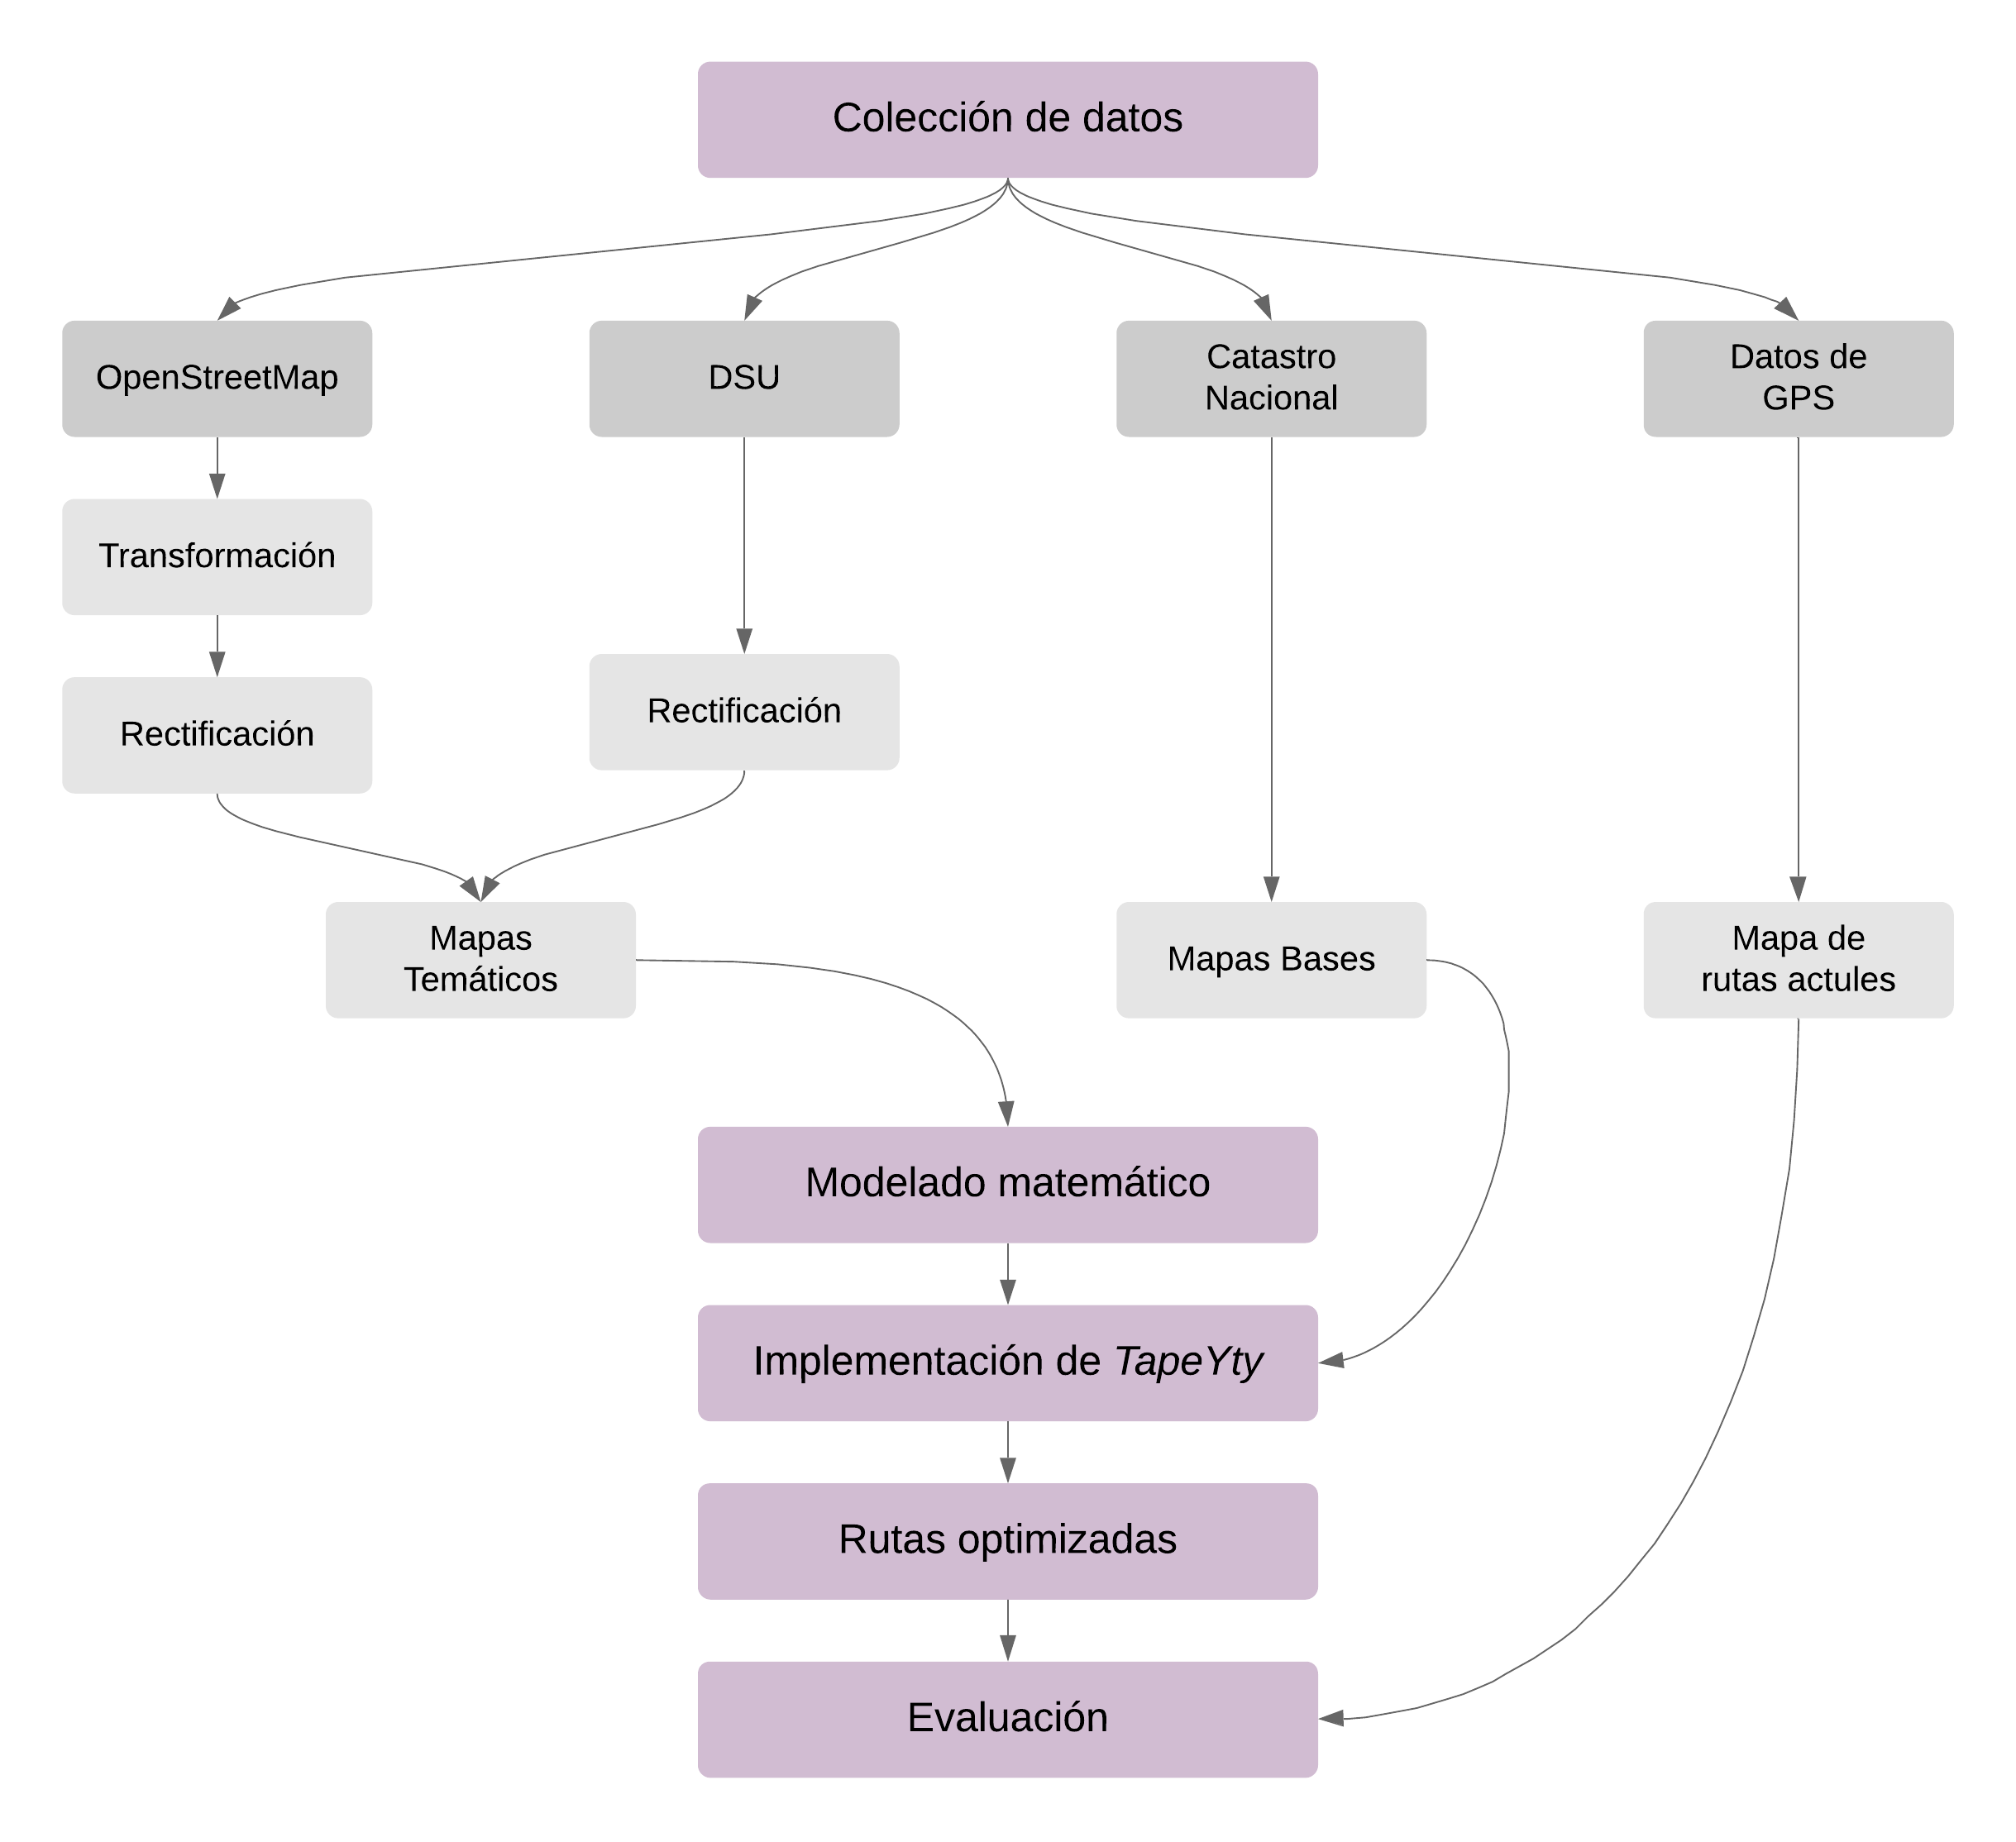
\includegraphics[width=\textwidth]{DiagramaDeMetodologia.png}}
\caption{Vista general de los procesos de la metodología aplicada.}
\label{fig:metodologia}
\end{figure}

% La solución del trabajo de investigación es lo que se buscará encontrar en el transcurso del desarrollo del TFG. La solución encontrada debe permitir obtener mejores resultados en cuanto a costo de recolección, en comparación a la situación actual en la DSU del municipio de Asunción, así como también, generar resultados óptimos que contribuyan con el estado del arte actual

\section{Colección de Datos}

Para visualizar y analizar las rutas de recolección es necesario contar con un mapa de calles y otro de zonas de recolección definidas por la DSU. Tanto el mapa de zonas como el de calles deben estar almacenados en la base de datos GIS para ser posteriormente utilizados durante el procesamiento de \textit{TapeYty}. Se crea una base de datos espacial utilizando el gestor de base de datos de código abierto PostgreSQL en su versión 10.8 \citep{PostgreSQL}, junto con su extensión PostGIS en su versión 2.4 \citep{PostGIS}, la cual brinda soporte para objetos geográficos.

Primeramente, se obtuvieron los datos de calles de la ciudad de Asunción usando como fuente OpenStreetMap (OSM), debido a que no se identificó una fuente institucional que proveyera de mapas de calles de la ciudad con sus sentidos. A continuación se detallan los pasos seguidos para obtener la red de rutas utilizada: 
\begin{enumerate}
    \item Se utiliza la herramienta \textit{osm2pgsql} para importar los datos de OSM a la base de datos, en el sistema de referencia geográfico WGS84 (SRID 4326). 
    \item Se utilizan las funciones de PostGIS para convertir los valores de latitud y longitud al tipo de dato geométrico \textit{Point}. 
    \item Las calles de OSM están representadas por líneas, que a su vez contienen una serie de nodos (puntos). Se excluyen los puntos que no pertenecen a calles de la ciudad, además de puntos superpuestos.
    \item Para un mejor manejo de la red de rutas se crea un proceso de segmentación de las calles, donde cada segmento de calle está formado por pares de nodos consecutivos, se define el sentido del segmento, longitud y si corresponde o no a un callejón sin salida.
    \item Por último, se realizan las transformaciones correspondientes para almacenar las restricciones de giro y contramano, desde los datos registrados en OSM.
\end{enumerate}

Para almacenar la información de red de calles se definen las siguientes tablas en la base de datos GIS:

\begin{itemize}
    \item \textbf{Nodo:} En esta tabla se almacenan los puntos que se utilizan como extremos de los segmentos de calle. Se almacena la latitud y la longitud.
    \item \textbf{Segmento:} Contiene líneas de calle formada a partir de dos nodos consecutivos. Se almacena el nombre, el nodo origen, el nodo destino, si es de único de sentido y si es sin salida. Si el segmento es de único sentido, entonces el nodo origen y destino definen el sentido del mismo.
\end{itemize}

Al importar los datos desde OSM se detectaron algunos datos incorrectos que generarían inconvenientes para la obtención del recorrido para la recolección de residuos. OSM identifica las calles sin salida por medio del atributo \textit{no\_exit}. Si su valor es \textit{true} representa una calle sin salida, sin embargo muchas calles sin salida lo tienen como \textit{false}. Otra inconsistencia encontrada es con el valor del atributo \textit{one\_way}, donde muchas calles sin salida tienen su valor en \textit{true} indicando que es de único sentido cuando realmente deben ser doble sentido.

Los problemas de datos mencionados fueron solucionados con sentencias SQL. Para identificar las calles sin salida se realizó una consulta donde se obtenga la unión de: ``todos los segmentos que tengan un nodo inicial que no sea nodo final ni inicial de algún otro segmento'' y ``todos los segmentos que tengan un nodo final que no sea inicial o final de otro segmento''. Se obtuvo como resultado la lista de todos los ID (identificadores) de los segmentos sin salida y se almacena en una tabla temporal. Se actualizan los campos de sin salida y sentido de todos aquellos segmentos cuyos ID se encuentran en la tabla temporal.

La delimitación de las zonas de recolección fue proveída por la DSU a través de un archivo \textit{shape} del tipo de dato geométrico \textit{Polygon}. Se realizan los siguientes procedimientos para la limpieza y corrección de los datos geográficos sobre dicha capa:

\begin{enumerate}
\item Se importa el \textit{shape} de Zonas a la base de datos mediante la herramienta \textit{shp2pgsql}, creándose así la tabla de zonas.
\item Se utiliza la opción de autoensamblado de QGIS. Esta opción ayuda a hacer coincidir con precisión los límites de las zonas con las calles de OSM.
% \item Con el programa QGIS, se agregan las capas PostGis de Segmentos, Nodos (de los segmentos) y la nueva de Zonas.
% \item Se configura la opción de autoensamblado de QGIS. Esta opción ayuda para hacer coincidir con precisión la edición de capas con los nodos de los segmentos. Es decir, se utilizan los nodos de los segmentos para hacer coincidir con los nodos de las líneas que formarán el polígono de la zona.
\item En la tabla de zonas se almacenan: nombre, superficie, densidad poblacional, cantidad de lotes y distrito.
\end{enumerate}

Para actualizar la superficie se utiliza la función geométrica de área de polígonos. Para actualizar la cantidad de lotes y distrito se utiliza la función de intersección. No se cuentan con datos de densidad poblacional de todas las zonas de recolección.

Los mapas bases de Departamentos y Distritos son proveídos a la aplicación por el Servicio Nacional de Catastro (SNC) a través de su portal de datos abiertos.

La DSU cuenta en algunos vehículos de su flota con un sistema de monitoreo mediante GPS: 

\begin{itemize}
    \item Se accede a los datos a través de archivos en formato de plantilla.
    \item Esta información es utilizada para el análisis y comparación de los resultados.
\end{itemize}

\section{Modelo matemático}

Como resultado de la revisión del estado del arte, se utiliza la solución propuesta por \citet{Braier2017AnArgentina} para optimizar el enrutamiento de vehículos recolectores, ya que este modelo contempla las restricciones de la red de rutas, resolviendo una de las debilidades de los enfoques de la programación matemática mencionado en \cite{Sulemana2018OptimalMethods}. Además, la falta de datos relacionados con la cantidad de toneladas recolectadas por zonas fue otro de los principales motivos por el cual se seleccionó un problema de ruta cuya demanda se encuentra sobre los arcos (calles que deben ser visitadas), y además no posea restricciones de capacidad.

El estudio en \cite{Braier2017AnArgentina} presenta similitudes con el caso de estudio de este trabajo, entre ellas es posible citar:

\begin{itemize}
    \item División de la ciudad en sectores y recolección casa por casa: La situación es muy similar, ya que el procedimiento consiste en recoger los residuos domiciliarios casa por casa, debiendo cubrir todas las calles de un conjunto de cuadras o manzanas, denominadas zonas.
    \item Tamaño de problema: Una zona de recolección abarca en promedio el mismo número (entre 40 y 80 cuadras aproximadamente).
    \item Calles, carreteras, caminos: el trabajo de \citet{Braier2017AnArgentina} tomó como caso de estudio la ciudad de Morón el cuál presenta caminos con particularidades muy comunes a otras sudamericanas como la de Asunción: calles sin salida, calles estrechas, peatonales, giros prohibidos, entre otros.
\end{itemize}

Los siguientes supuestos son establecidos:

\begin{itemize}
    \item El vehículo recolector cuenta con capacidad suficiente para recoger los residuos de una zona determinada.
    \item El tráfico es constante en una zona de trabajo en el turno en que se recogen sus residuos.
    \item Las modificaciones geográficas de los datos espaciales estarán a cargo de una persona capacitada en el área GIS.
    % La persona encargada de la administración del sistema posee conocimientos básicos en GIS y podrá actualizar, crear y eliminar una zona de trabajo mediante el sistema \textit{QGis}
\end{itemize}

Cada zona de recolección de la ciudad de Asunción es representada por un grafo mixto $H$ \citep{Braier2017AnArgentina}, cuyos nodos representan las esquinas de las calles en la zona, y los arcos son los segmentos de calles que corren entre dos intersecciones consecutivas. Las calles de un único sentido están representadas por arcos dirigidos y las calles finas de doble sentido por arcos no dirigidos, ya que ambos lados de la calle pueden ser servidos en un solo viaje. En el caso de calles anchas de doble sentido, como las avenidas, cada lado debe ser servido de forma separada, por lo que estas calles se representan con dos arcos dirigidos, una en cada sentido.

Para incorporar las restricciones de regulación de tráfico se construye un grafo dirigido $G'$ desde el grafo $H$. El grafo $H$ es expandido dividiendo cada nodo en varios nuevos nodos representando todas las formas en las que se puede llegar y salir de la esquina en cuestión. En la Figura \ref{fig:grafo_expandido}(a) se puede observar un nodo en el grafo original $H$ antes de su expansión y en la Figura \ref{fig:grafo_expandido}(b) el nodo que ha sido expandido en seis nuevos nodos, representando cada posible entrada y salida del nodo. Los arcos auxiliares dirigidos son agregados y conectan los nuevos nodos, representando así las transiciones permitidas de una esquina a otra.

El modelo de programación entera propuesto por \citet{Braier2017AnArgentina} está definido de la siguiente manera:

\subsection{Conjuntos y Parámetros}
\label{sec:conjunto-parametros}

\begin{itemize}
\item $G'(V, A)$: Grafo dirigido en el que los nodos V corresponden a todas las alternativas posibles para llegar a las esquinas de las intersecciones y A está compuesto por arcos que se pueden atravesar en una sola dirección específica.

\item $E \subseteq \{ \{i, j\}: i \in V, j \in V, i \neq j\}$: Representan segmentos de calles de dos vías que pueden ser recorridos en cualquier sentido.

\item $AM \subseteq A $: Arcos obligatorios que representan segmentos que deben recorrerse únicamente en el sentido especificado.

\item $w : A \rightarrow \mathbb{R} $: Función de peso que asocia un peso a cada arco, en este caso la longitud del segmento de calle. Los arcos auxiliares entre nodos que representan esquinas tienen un mismo valor ínfimo.

\item $I \subseteq V $: Nodos que especifican los puntos de inicio permitidos para la ruta.

\item $\mathcal{S} \subseteq V$: Se define $\delta^+ (\mathcal{S}) = \{i j \in A: i \in S , j \notin \mathcal{S} \}$ , que representa un conjunto de arcos que van desde nodos en $\mathcal{\mathcal{S}}$ a nodos en $V \backslash \mathcal{S}$.
\end{itemize}

El problema de ruteo es una versión particular del problema del cartero rural abierto dirigido generalizado, ya que el arco $i j \in E $ determina el grupo de arcos $L_{i j} = \{i j, j i\}$, en el que al menos uno de ellos debe ser atravesado en la solución final y además se busca un camino cuyo nodo inicial y final no se especifican.

\begin{figure}[tbp]
\centerline{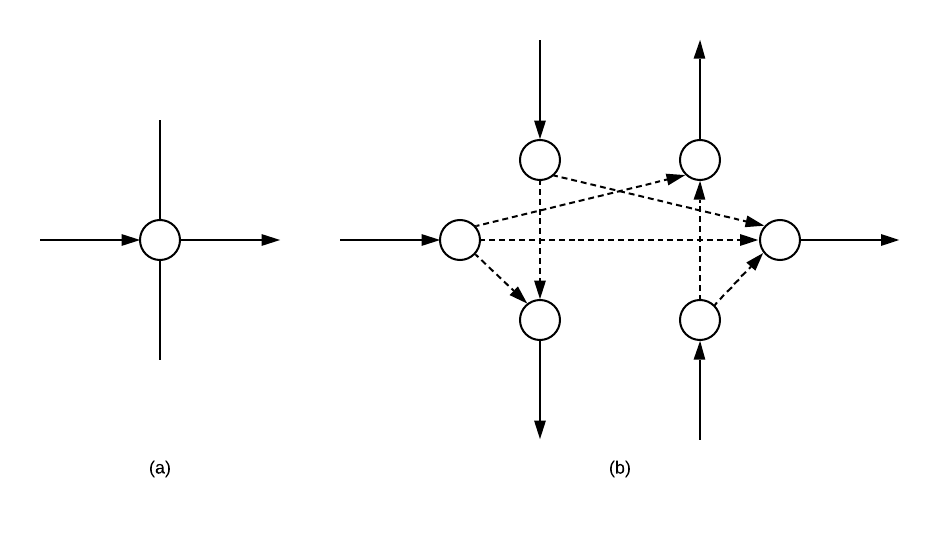
\includegraphics[width=9.5cm]{expanded_graph.png}}
\caption{Expansión de un cruce entre una calle de sentido único y una calle de doble sentido. (a) Grafo mixto original $H$. (b) Grafo dirigido $G'$ luego de la expansión, los arcos auxiliares están representados por líneas discontinuas. [Fuente: \citet{Braier2017AnArgentina}]}
\label{fig:grafo_expandido}
\end{figure}

\subsection{Variables de decisión}
\begin{itemize}
\item $x_{i j}$: Para cada arco $ {i j} \in A$ esta variable representa el número de veces que $i j$ es atravesado.

\item $s_i$: Para cada nodo $i \in I$ esta variable binaria especifica si  $i$ es el primer nodo de la ruta.

\item $t_j$: Para cada nodo $j \in V$ esta variable binaria indica si $j$ es el último nodo de la ruta.
\end{itemize}

\subsection{Definición del programa entero}
\label{sec:programa-entero}
\begin{equation*} \tag{0} \label{eq0}
\min \sum_{i j \in A} w_{i j} x_{i j}  \\
\end{equation*} 
\hbox{}

\begin{equation} \tag{1} \label{eq1}
\begin{gathered}
x_{i j} \geq 1 \\
\forall i j \in A M
\end{gathered}
\end{equation} 
\hbox{}

\begin{equation} \tag{2} \label{eq2}
\begin{gathered}
x_{i j} + x_{j i} \geq 1 \\
\forall i j \in E
\end{gathered}
\end{equation}
\hbox{}

%ecuacion 3a
\begin{equation} \tag{3a} \label{eq3a}
\begin{gathered}
s_i + \sum_{j: j i \in A} x_{j i} = \sum_{j: i j \in A} x_{i j} + t_i \\
\forall i \in I
\end{gathered}
\end{equation} 
\hbox{}

%ecuacion 3b
\begin{equation} \tag{3b} \label{eq3b}
\begin{gathered}
\sum_{j: j i \in A} x_{j i} = \sum_{j: i j \in A} x_{i j} + t_i \\
\forall i \in V\backslash I
\end{gathered}
\end{equation}
\hbox{}

\begin{equation} \tag{4} \label{eq4}
\sum_{i \in I} s_i = 1 
\end{equation}
\hbox{}

\begin{equation} \tag{5} \label{eq5}
\sum_{i \in V} t_i = 1 
\end{equation}
\hbox{}

\begin{equation} \tag{6} \label{eq6}
\begin{gathered}
    \sum_{i j \in \delta + (\mathcal{S})} x_{i j} \geq 1 \\
    \forall \mathcal{S} \subseteq V
\end{gathered}
\end{equation}
\hbox{}

\begin{equation} \tag{7} \label{eq7}
\begin{gathered}
    x_{i j} \in \mathbb{Z}_+ \\
    \forall i j \in A
\end{gathered}
\end{equation}
\hbox{}

\begin{equation} \tag{8} \label{eq8}
\begin{gathered}
    s_i \in \{0,1\} \\
    \forall i \in I
\end{gathered}
\end{equation}
\hbox{}

\begin{equation} \tag{9} \label{eq9}
\begin{gathered}
    t_i \in \{0,1\} \\
    \forall i \in V
\end{gathered}
\end{equation}

La función objetivo (\ref{eq0}) busca minimizar el costo total de la ruta de recolección de residuos en una zona. El costo en este trabajo se refiere a la distancia recorrida por el vehículo recolector. La restricción (\ref{eq1}) impone que todos los arcos de único sentido deben ser visitados al menos una vez, la (\ref{eq2}) requiere que los arcos no dirigidos sean atravesados al menos una vez en cualquier sentido. Las restricciones (\ref{eq3a}) y (\ref{eq3b}) aseguran que la solución encontrada es realmente un camino agregando la condición de conservación de flujo estándar a cada nodo. Las restricciones (\ref{eq4}) y (\ref{eq5}) garantizan que el nodo inicial y final sean únicos. Las restricciones (\ref{eq1})-(\ref{eq5}) permiten la formación de subtours, la restricción (\ref{eq6}) es el estándar de eliminación de subtours. Las restricciones (\ref{eq7})-(\ref{eq9}) especifican los valores posibles para las variables del modelo.

\subsection{Algoritmo de solución}
\label{algoritmo-solucion}
% En el modelo dado en la sección \ref{sec:programa-entero} se puede observar la restricción de eliminación de subtours la cual es muy costosa en la generación de las mismas como también en  la complejidad del problema. En este contexto la estrategia propuesta en \cite{Braier2017AnArgentina} se basa en tratar de obtener una solución rápidamente sin considerar el problema de subtour e ir agregando las restricciones sucesivamente, esto se conoce como técnica de agregación dinámica de restricciones a un modelo relajado.

En el modelo dado en la sección \ref{sec:programa-entero} se puede observar la restricción de eliminación de subtours la cual es muy costosa en la generación de las mismas como también en la complejidad del problema. En este contexto la estrategia propuesta en \citet{Braier2017AnArgentina} se basa en tratar de obtener una solución rápidamente sin considerar el problema de subtour, en caso de que existan subtours se eliminan mediante el procedimientos de mezcla de subtours, si no se puede utilizar esta técnica se van agregando las restricciones sucesivamente, esto se conoce como técnica de agregación dinámica de restricciones a un modelo relajado.

Los siguientes pasos detallan la estrategia:

\begin{enumerate}
\item Crear el modelo relajado $R: = (\ref{eq1}) - (\ref{eq5})$ y $(\ref{eq7}) - (\ref{eq9})$.
\item Resolver $R$.
\item Si no se puede encontrar ninguna solución para $R$, retornar ``infactible'' y parar.
\item Si la mejor solución encontrada para $R$ no tiene subtours, retornar esta solución y parar.
\item Si los subtours pueden ser mezclados con el tour que contiene el nodo inicial y final, entonces mezclarlos, retornar la solución obtenida y parar.
\item De lo contrario, agregar a $R$ la restricción de eliminación de subtour estándar (\ref{eq6}) por cada subtour en la solución y regresar al Paso 2.
\end{enumerate}

El procedimiento de mezcla de subtours descrito por \citet{Braier2017AnArgentina}, utilizado en el paso 5, consiste en que dado un subtour \textit{T} y el camino principal \textit{P}, es decir el camino que empieza en el único vértice $i \in I$ con $s_i = 1$, y termina respectivamente en $t_i = 1$, se intenta intercambiar los arcos auxiliares para mezclar \textit{T} y \textit{P}. Se puede presentar una de las siguientes tres configuraciones:

\begin{itemize}
    \item Configuración A: Si el camino principal y el subtour se encuentran en algún nodo intermedio, como en la Figura \ref{fig:procedimiento_mezcla_subtours}(a), entonces son unidos como en la Figura \ref{fig:procedimiento_mezcla_subtours}(b)
    \item Configuración B: Si el subtour se encuentra con el último nodo en la ruta principal, como en la Figura \ref{fig:procedimiento_mezcla_subtours}(c), entonces se unen como en la Figura \ref{fig:procedimiento_mezcla_subtours}(d).
    \item Configuración C: Si el subtour se encuentra con el primer nodo en la ruta principal, como en la Figura \ref{fig:procedimiento_mezcla_subtours}(e), entonces se unen como en la Figura \ref{fig:procedimiento_mezcla_subtours}(f).
\end{itemize}

\begin{figure}[tbp]
\centerline{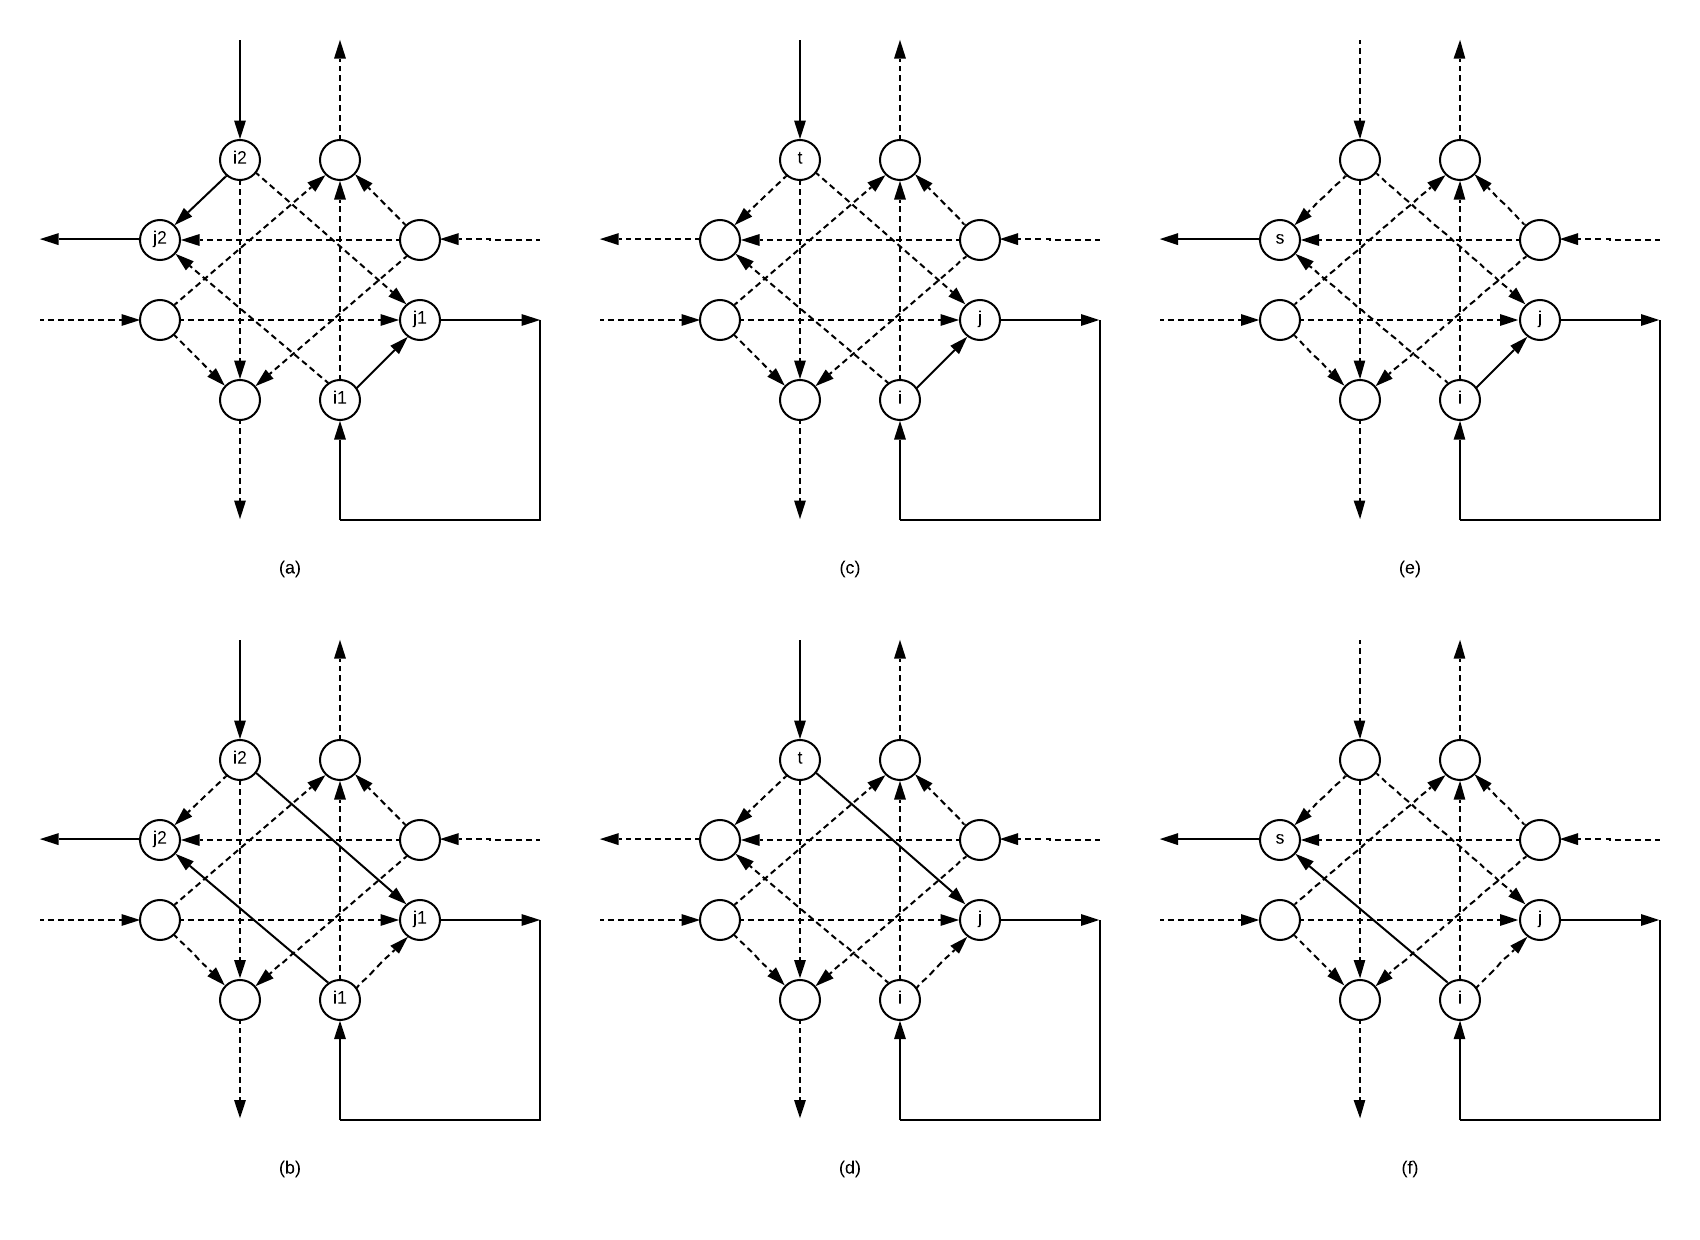
\includegraphics[width=\textwidth]{mezcla_subtours.png}}
\caption{Posibles configuraciones en el procedimiento de la mezcla de subtours. Si \textit{P} y \textit{T} tienen la configuración (a), (b) o (c), entonces la solución es modificada de acuerdo a lo especificado en (b), (d) o (f) respectivamente. [Fuente: \citet{Braier2017AnArgentina}]}
\label{fig:procedimiento_mezcla_subtours}
\end{figure}

Este procedimiento es aplicado para cada subtour en la solución hasta que todos sean mezclados al camino principal, dado que el costo de todos los arcos auxiliares que unen los nodos de las esquinas es el mismo, la ruta modificada permanece óptima, por lo que el algoritmo se detiene y devuelve la solución obtenida en este caso.

Dado que no siempre los subtours pueden ser mezclados con la técnica recién mencionada, el algoritmo principal descrito agrega una restricción estándar de eliminación de subtours al modelo $R$, tal y como se especifica en el Paso 6.

Finalmente, en caso que el modelo matemático encuentre una solución factible, el resultado del modelo indica la distancia total, los arcos que son atravesados y el número de veces que estos son atravesados. Sin embargo, para conocer el camino a seguir es necesario encontrar la secuencia del mismo. 

\section{Método de secuenciación}

% En este trabajo se realiza una búsqueda en profundidad para obtener la secuencia a seguir a partir del resultado del problema descrito en la sección anterior. El algoritmo toma como entrada el nodo inicial, nodo final y la cantidad de veces que se atraviesa por cada arco del grafo $G$. Se describe a continuación los pasos del algoritmo:

% En este trabajo se realiza una búsqueda en profundidad para obtener la secuencia a seguir a partir del resultado del problema descrito en la sección anterior. El algoritmo recibe como parámetros de entrada el nodo inicial, nodo final, la cantidad de veces que se atraviesa por cada arco del grafo $G$ y un grafo dirigido $N$ construido teniendo en cuenta solo los arcos atravesados. Se describe a continuación los pasos del algoritmo:

% \begin{enumerate}
% \item Leer el grafo $N$ resultante del GDRPP abierto. 
% \item Inicializar nodo actual al valor del nodo inicial.
% \item Inicializar un vector vacío $seq$, en el que los nodos se almacenarán en el orden en que deben ser visitados.
% \item Agregar a $seq$ el nodo actual.
% \item Si el nodo actual es igual al nodo final y ya se atravesaron todos los arcos, entonces retornar $seq$ y parar.
% \item Sino, tomar uno de los nodos sucesores del nodo actual en $N$, donde el arco formado por el nodo actual y el nodo sucesor aún no haya sido tenido en cuenta, asignar como nodo actual el nodo sucesor y volver al paso 4.
% \end{enumerate}

En este trabajo se utiliza el algoritmo implementado en \cite{RiveraHazim2015APath} que encuentra el camino euleriano de un multigrafo dirigido para obtener la secuencia a seguir. Se genera un multigrafo dirigido $MG$ a partir del resultado del problema descrito en la sección anterior, creando arcos dirigidos según la cantidad de veces que se atraviesa por cada arco del grafo $G'$ . 

El algoritmo recibe como parámetros de entrada el nodo inicial, nodo final y $MG$. Devuelve como resultado, la secuencia de arcos del recorrido solución. Los siguientes pasos detallan el algoritmo de secuenciación:

\begin{enumerate}
    \item Comience con una pila vacía y un camino (euleriano) vacío. 
    \item Se halla el multigrafo reverso de $MG$ y se trabajo con el mismo. El reverso es un grafo con los mismos nodos y bordes pero con las direcciones de los arcos invertidas.
    \item Se elige el vértice que representa el nodo final.
    \item Si el vértice actual no tiene arcos salientes (es decir, vecinos): agréguelo al camino, elimine el último vértice de la pila y configúrelo como el actual. De lo contrario (en caso de que tenga arcos salientes, es decir, vecinos): agregue el vértice a la pila, tome cualquiera de sus vecinos, elimine el arco entre ese vértice y el vecino seleccionado, y establezca ese vecino como el vértice actual.
    \item Repita el Paso 4 hasta que el vértice actual no tenga más arcos salientes (vecinos) y la pila esté vacía.
\end{enumerate}

La complejidad del algoritmo es $O(N + M)$, donde $N$ es el número de vértices y $M$ es el número de arcos.

\section{Ejemplo Numérico}
A continuación se describe un ejemplo simple de cómo la aplicación produce la secuencia del camino a seguir desde el resultado generado por la programación matemática.

El Paso 1 de la Figura \ref{fig:PasosSolucion} muestra los datos de salida que genera el modelo matemático (Algoritmo  de  solución, sección \ref{algoritmo-solucion}) a partir de un resultado factible. La salida contiene todos los segmentos que son utilizados como solución junto con el número de veces que se recorre cada uno de ellos, así como también despliega los nodos que resultaron elegidos como nodo inicial y nodo final del recorrido. 

Posteriormente, con estos datos se procede a crear el multigrafo dirigido $MG$ con la cantidad total de arcos resultantes (Paso 2). El multigrafo generado pasa a formar parte de la entrada, junto con los nodos inicial y final, para obtener la secuencia del camino a seguir (Paso 3). Por último, el algoritmo de secuenciación se resuelve y genera como salida la secuencia de arcos del algoritmo de optimización.

\begin{figure}[tb]
\centerline{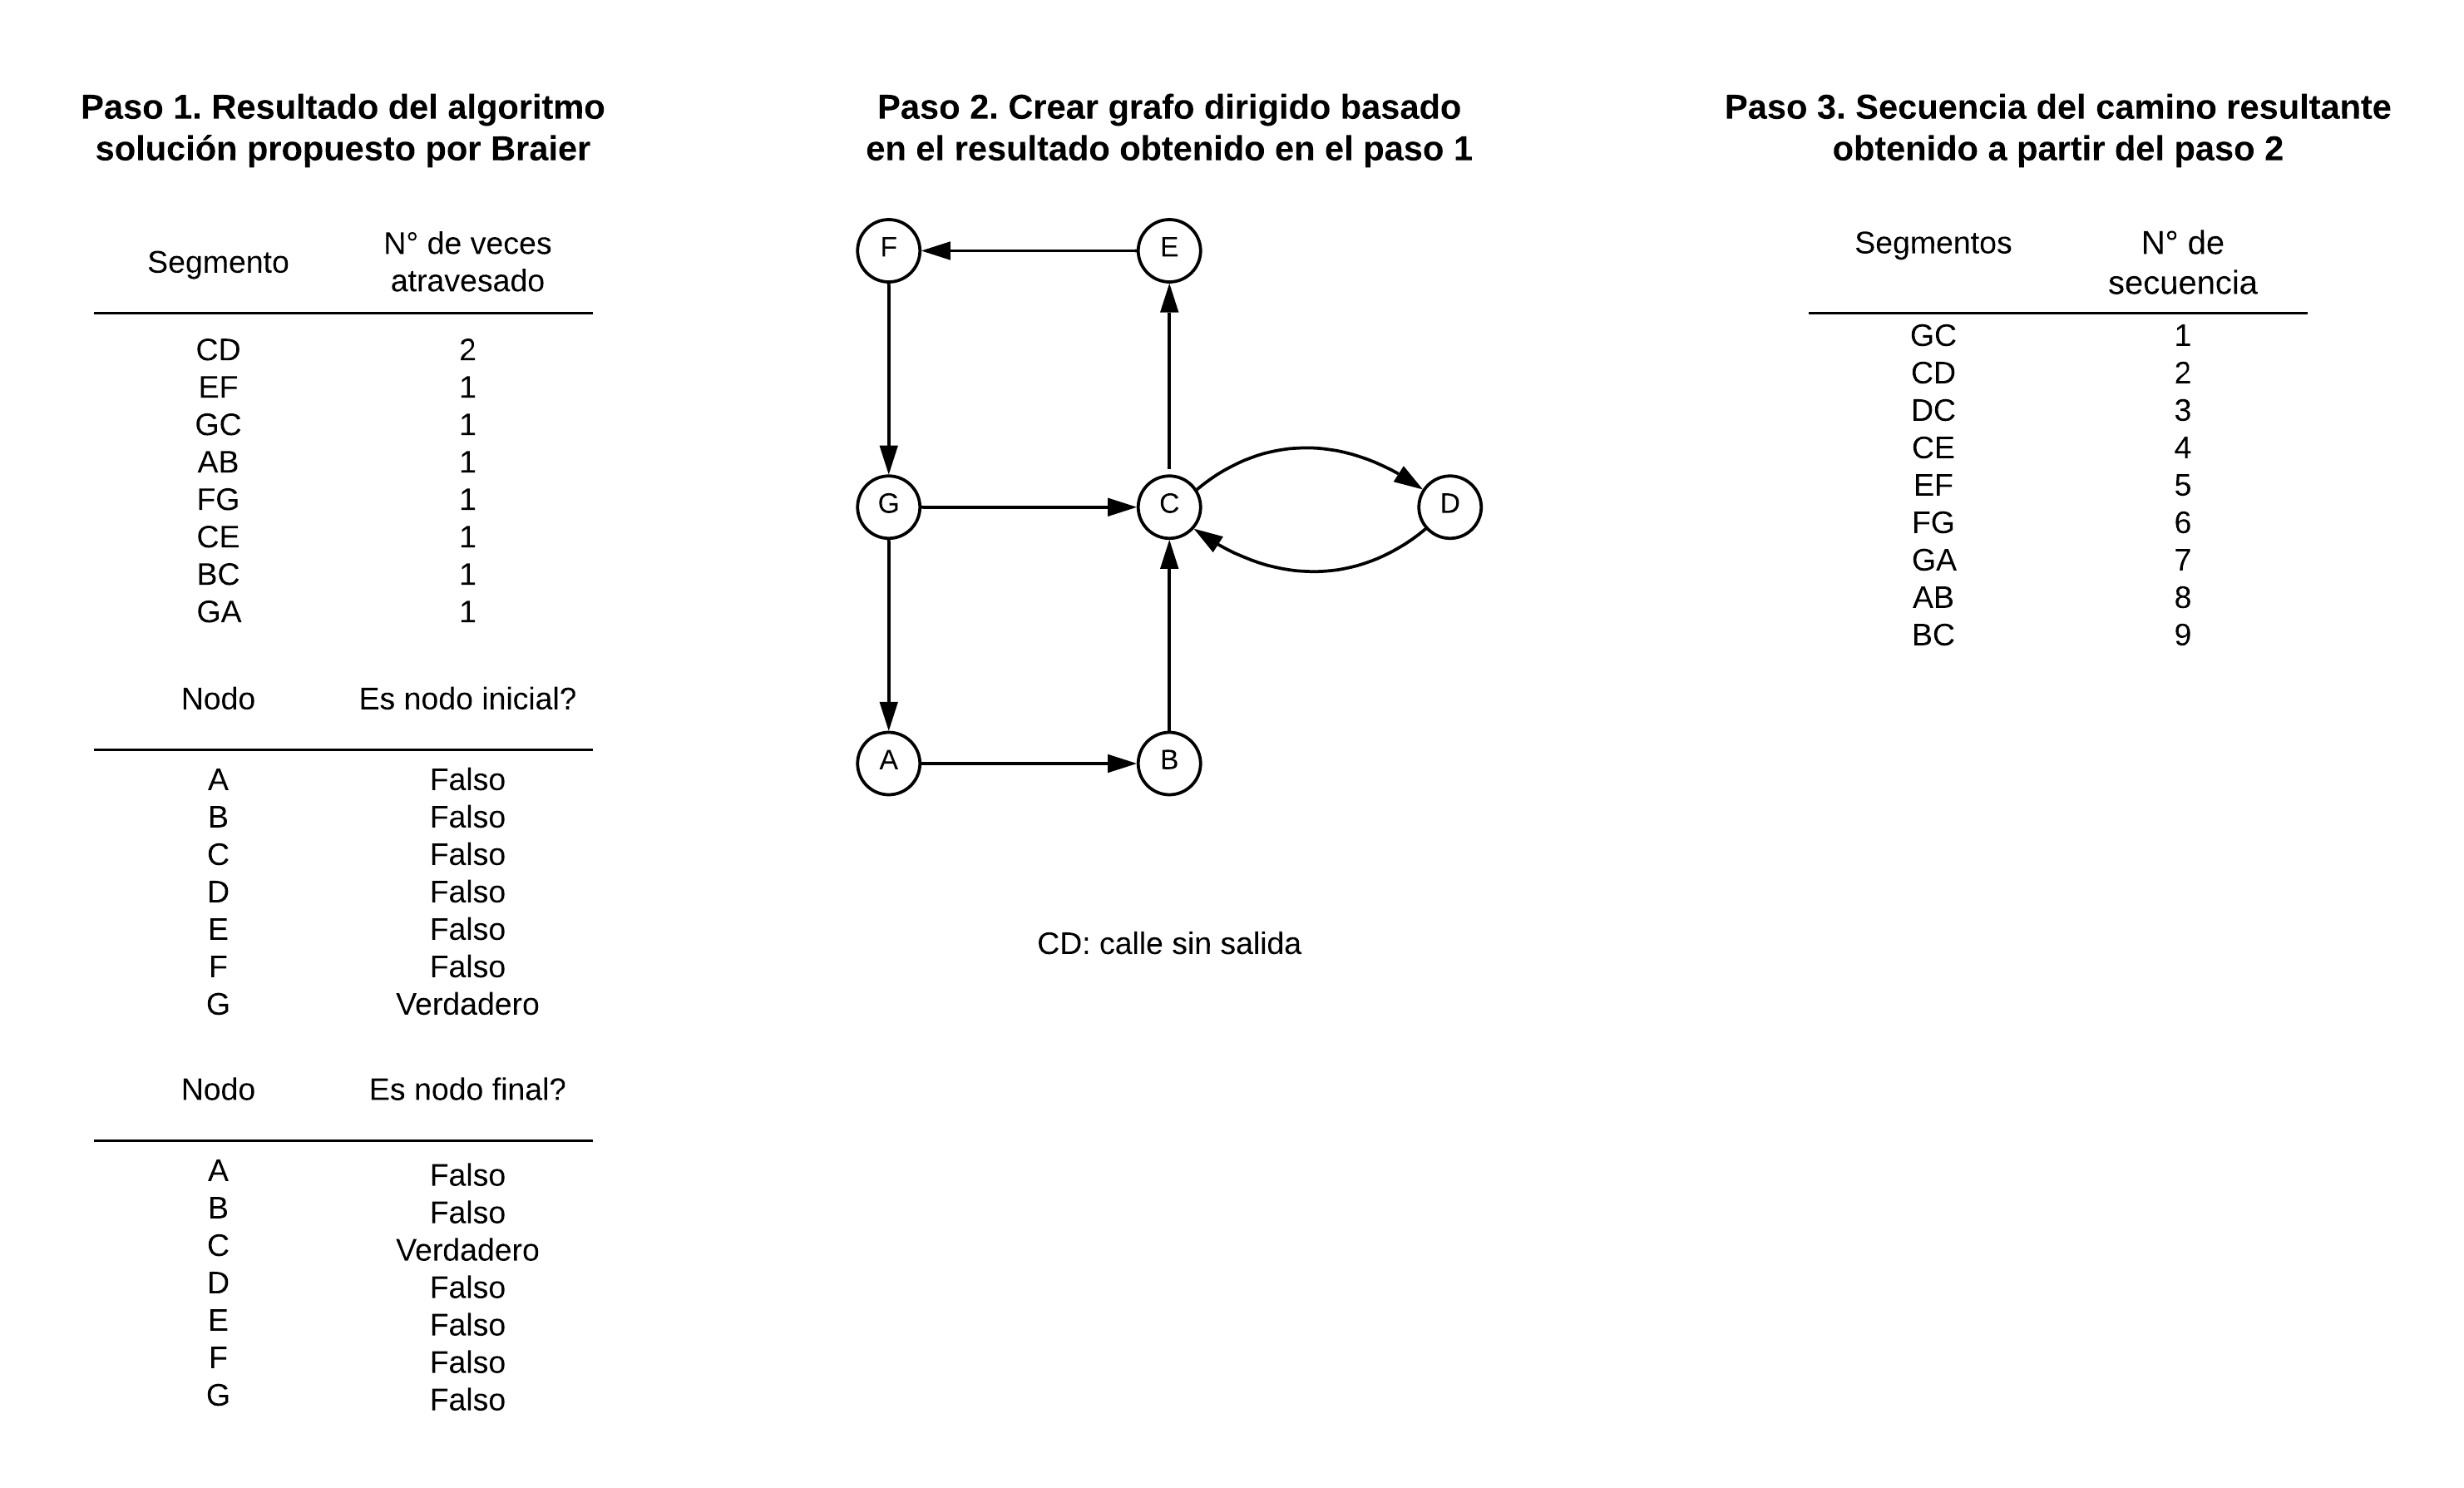
\includegraphics[width=\textwidth]{pasos_de_solucion.png}}
\caption{Pasos de solución para obtener la secuencia del camino del vehículo recolector en una zona}
\label{fig:PasosSolucion}
\end{figure}


